\documentclass[final]{beamer}

% Beamer poster
\mode<presentation>{\usetheme{icassp2019}}
\usepackage[orientation=landscape,size=a0,scale=1.31]{beamerposter}
\setbeamertemplate{itemize subitem}{\mybf{--}}
% \setbeamertemplate{itemize subitem}{\raisebox{0.12ex}{$\blacktriangleright$}\hskip0.1em}
\definecolor{tablue20blue}{RGB}{31,119,180}
\definecolor{tablue20orange}{RGB}{255,127,14}
\definecolor{tablue20red}{RGB}{214,39,40}
\definecolor{tablue20green}{HTML}{2ca02c}
\newcommand{\nonparallel}[1]{\textcolor{tablue20orange}{#1}}
\newcommand{\goal}[1]{\textcolor{tablue20orange}{#1}}
\newcommand{\zeroshot}[1]{\textcolor{tablue20blue}{#1}}
\newcommand{\realtime}[1]{\textcolor{tablue20red}{#1}}
\newcommand{\highqual}[1]{\textcolor{tablue20green}{#1}}

\definecolor{softgreen}{RGB}{25, 168, 34}
\definecolor{softred}{RGB}{188, 26, 11}

\usepackage{booktabs}
\usepackage{tabularx}
\usepackage{multirow}

\newcommand{\mytable}{
    \centering
    \small
    \renewcommand{\arraystretch}{1.2}
    }
\renewcommand{\tabularxcolumn}[1]{m{#1}}
\newcolumntype{C}{>{\centering\arraybackslash}X}
\newcolumntype{L}{>{\raggedright\arraybackslash}X}
\newcolumntype{R}{>{\raggedleft\arraybackslash}X}
\newcolumntype{P}[1]{>{\raggedright\arraybackslash}p{#1}}
\usepackage{siunitx}
\sisetup{detect-all}
\usepackage{etoolbox}                           % bold fonts in table
\newcommand{\ubold}{\fontseries{b}\selectfont}  % bold fonts in table
\robustify\ubold                                % bold fonts in table
\newcommand{\tablecaptionsep}{\vspace*{-0pt}}

% Graphics
\graphicspath{{fig/}}

% Mathematics
\usefonttheme[onlymath]{serif}
% \usefonttheme{serif}
\renewcommand{\vec}[1]{\boldsymbol{\mathbf{#1}}}

% Colours
\newcommand{\graybf}[1]{\textcolor{darkestgray}{\textbf{#1}}}
% \newcommand{\mybf}[1]{\textbf{#1}}
\newcommand{\mybf}[1]{\textcolor{darkestgray}{\textbf{#1}}}

% Layout
\newlength{\columnheight}
% \setlength{\columnheight}{66.25cm} % landscape
\setlength{\columnheight}{66.25cm} % landscape
% \setlength{\columnheight}{65.5cm} % landscape
% \setlength{\columnheight}{103cm} % portrait

% Tables
\usepackage{booktabs}
\usepackage{tabularx}
% \newcommand{\mytable}{\centering
                    %   \renewcommand{\arraystretch}{1.05}
                    %   }
\newcolumntype{C}{>{\centering\arraybackslash}X}
\newcolumntype{L}{>{\raggedright\arraybackslash}X}
\newcolumntype{R}{>{\raggedleft\arraybackslash}X}
\renewcommand{\tabularxcolumn}[1]{m{#1}}

% Text
\newcommand{\system}[1]{{\footnotesize \textsc{#1}}}

% Title and author
\title{A Temporal Extension of \\Latent Dirichlet Allocation for \\Unsupervised Acoustic Unit Discovery}
\author{Werner van der Merwe, Herman Kamper, Johan du Preez}
\institute{MediaLab, E\&E Engineering, Stellenbosch University, South Africa}

\begin{document}

\begin{frame}[t]
\begin{columns}[T]

\begin{column}{.01\linewidth}\end{column} % border column


\begin{column}{.33\linewidth}
\centering
\begin{minipage}[T]{.97\textwidth}\parbox[t][\columnheight]{\textwidth}{

% ================================
%  BACKGROUND BLOCK
% ================================
\begin{block}{Unsupervised acoustic unit discovery}

    % \begin{itemize}
    %     \setlength{\itemsep}{0.5ex}
    %     \item Voice conversion (VC) can be used to augment training data of automatic speech recognition (ASR) systems:
    % \end{itemize}
    
    % % \vspace{1ex}
    
    % \begin{columns}[c]
    %     \column{.01\textwidth}
        
    %     \column{.98\textwidth}
    %     \begin{center}
    %         % 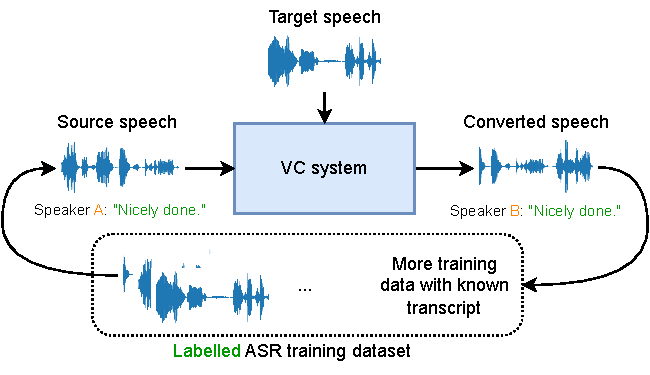
\includegraphics[width=0.7\textwidth]{figures/data_aug_diagram.pdf}
    %          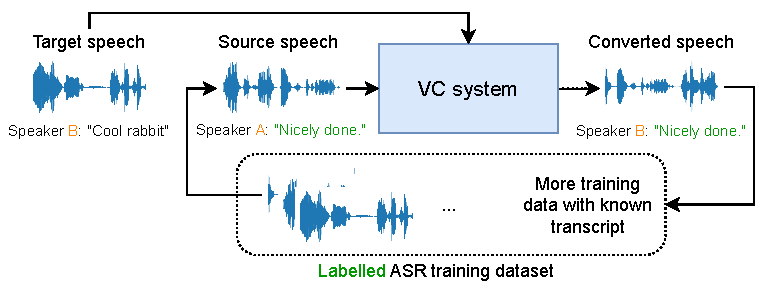
\includegraphics[width=1.0\textwidth]{figures/data_aug_diagram_v2.pdf}
    %     \end{center}
        
    %     \column{.01\textwidth}
    % \end{columns}
    
    % \vspace{1ex}

    % \begin{itemize}
    %     \setlength{\itemsep}{0.5ex}
        
    %     \item Attempts using VC for English ASR augmentation have met limited success.
    %     \item ASR still struggles in very low-resource settings with $<1$~h of labeled speech.
    %     \item \mybf{Research question:} can we design a VC system which can be used cross-lingually to improve ASR performance in very low-resource settings?
        
    %     \item To be practically useful for ASR augmentation, it needs to:
        
    %     \begin{enumerate}
    %         % \item \nonparallel{be trainable with non-parallel data}
    %         \item \zeroshot{work on unseen languages and speakers (any-to-any VC model)}
    %         \item \realtime{run reasonably fast so that augmenting an entire dataset is feasible.}
    %         \item \nonparallel{retain high quality in low-resource settings} % \highqual = green
    %     \end{enumerate}
        
    %     % \item \mybf{Goal:} compare existing voice conversion (VC) models and attempt to develop a new model to better satisfy these requirements.
    % \end{itemize}
\end{block}


% \vfill

% \vfill

% ================================
%  COMPONENTS OF VC SYSTEMS
% ================================
\begin{block}{Vector-quantised neural networks}
    % \vspace{0.2cm}
    % % \begin{center}
    % %     \centerline{\includegraphics[width=1\linewidth, trim={0cm 0cm 2cm 0cm},clip]{fig2/vc-blockdiag.pdf}}
    % % \end{center}
    % % \vspace{-2.5cm}

    % \vspace*{-1.3cm}
    % \begin{columns}[c]
    %     \column{.01\textwidth}
        
    %     \column{.98\textwidth}
    %     \begin{center}
    %         \centerline{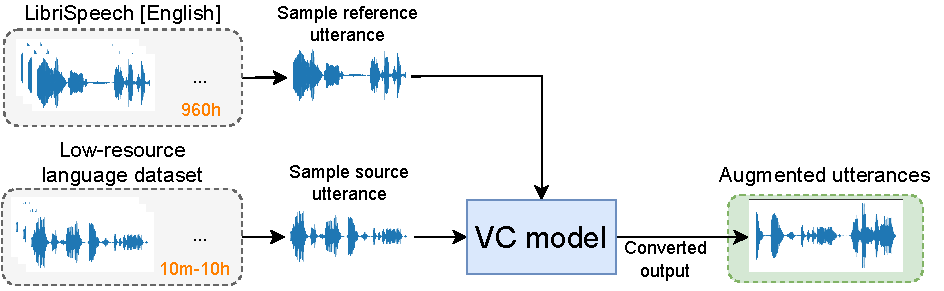
\includegraphics[width=0.9\textwidth,trim={0.0cm 0cm 0.0cm 0cm},clip]{figures/data_aug_cross_lingual.pdf}}
    %     \end{center}
        
    %     \column{.01\textwidth}
    % \end{columns}
    
    % \vspace{-0.3cm}

    % Combined \highqual{augmented} and original low-resource data now contains \\ \zeroshot{greater speaker diversity} $\implies$ improve ASR generalization.
    
\end{block}

% ================================
%  Experimental details
% ================================
\begin{block}{Latent Dirichlet allocation}
    % \begin{itemize}
    % \vspace{-0.5cm}
    %     \setlength{\itemsep}{0.5ex}
    %     \item \mybf{VC training:} use fixed pretrained \texttt{CPC-Big} encoder and train rest on non-parallel LibriSpeech 960~h training set.
    %     % \item \mybf{Pretrained networks:} use fixed \texttt{CPC-Big} model trained on English LibriSpeech.%\highqual{($\sim$9~min)}.
    %     \item \mybf{ASR setup:} use pretrained \texttt{XLSR-53} wav2vec 2.0 model, fine-tune with CTC on \highqual{labelled low-resource settings with varying amounts of augmented data}. No LM used in very low-resource settings -- unlikely to be available.
    %     \item \mybf{Low-resource settings}: simulated low-resource English baseline, final evaluations with 10~min of \zeroshot{Afrikaans, Setswana, isiXhosa, Sepedi} speech.
    % \end{itemize}
\end{block}

% % ================================
% %  HGST
% % ================================
% \begin{block}{Hierarchical global style tokens}
% Introduced by TODO in TODO as a way to separate speaker information from speech. 
%     \begin{center}
%         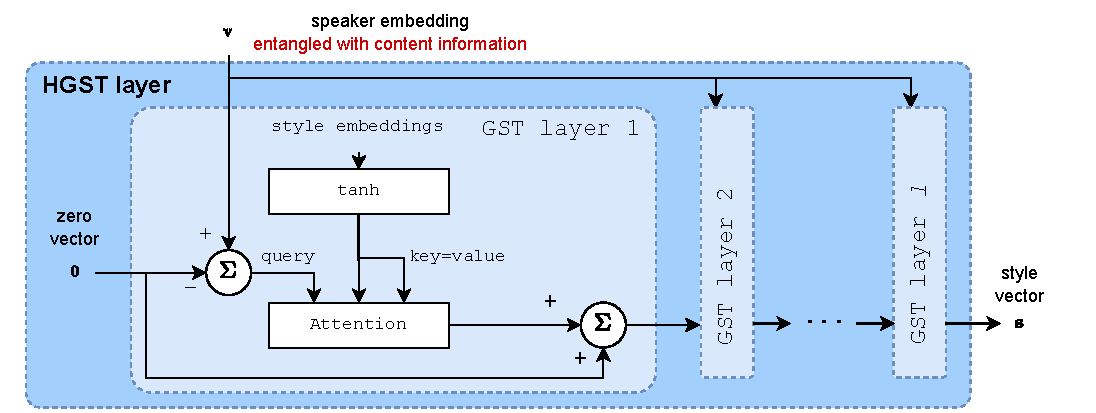
\includegraphics[width=0.7\linewidth]{figures/hgst.pdf}
%     \end{center}
%     % \centerline{\includegraphics[width=0.9\textwidth]{fig2/settings.pdf}}
% %     \centerline{\includegraphics[scale=2.75]{xlingual_keyword_spotting}}
% \end{block}

}\end{minipage}
\end{column}



\begin{column}{.33\linewidth}
\centering
\begin{minipage}[T]{.97\textwidth}\parbox[t][\columnheight]{\textwidth}{

% ================================
%  One-to-one models
% ================================
% \begin{block}{One-to-one models}
%     \centerline{\includegraphics[width=1\textwidth,trim={0.5cm 0cm 2cm 0cm},clip]{fig2/one-to-one-models.pdf}} %l b r t
% \end{block}

% \vfill

% ================================
%  Many-to-many models
% ================================
\begin{block}{Markov chain latent Dirichlet allocation}
    % \vspace*{-1.5cm}
    % \vspace*{-0.3cm}
    % \centerline{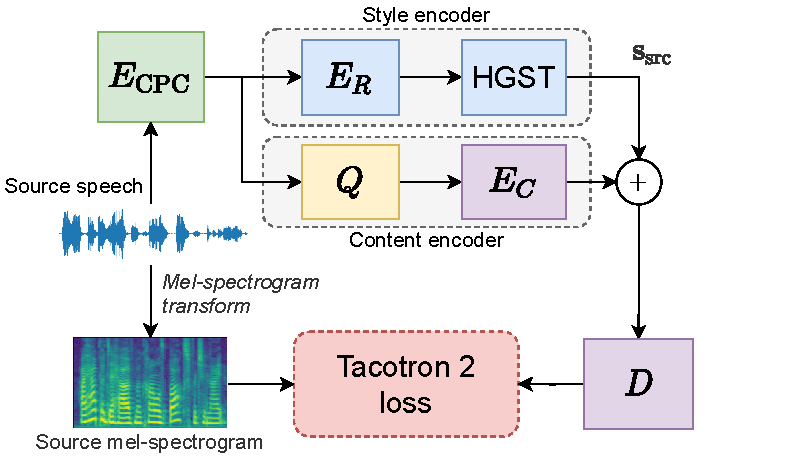
\includegraphics[width=0.75\textwidth]{figures/HGST12_training.pdf}}
    % \begin{itemize}
    %     % \vspace{-0.5cm}
    %     \setlength{\itemsep}{0.5ex}
    %     \item Style encoder isolates speaker identity in style vector $\mathbf{s}_{\text{src}}$; content encoder captures linguistic content as CPC feature sequence. 
    %     \item Self-supervised objective: $L_2$ loss between source and predicted mel-spectrogram from Tacotron 2 style decoder $D$.
    % \end{itemize}
\end{block}

\begin{block}{Experimental setup}
    % \vspace{-0.3cm}
    % \centerline{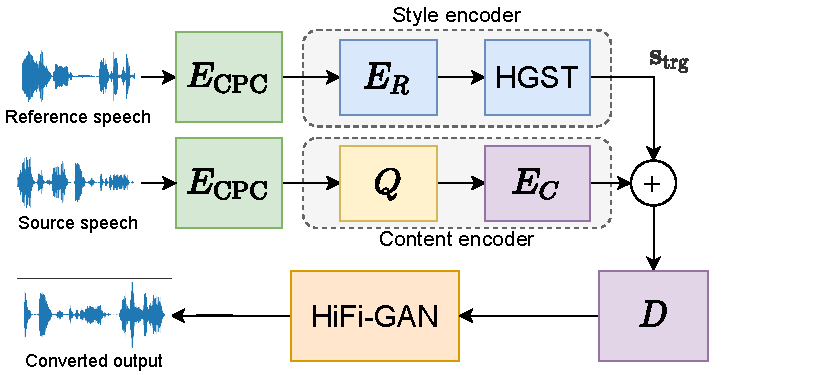
\includegraphics[width=0.75\textwidth]{figures/HGST12_inference.pdf}}

    % % \begin{columns}[c]
    % %     \column{.01\textwidth}
        
    % %     \column{.46\textwidth}
    % %     \begin{center}
    % %         Training setup
    % %         \vspace*{0.7cm}
    % %         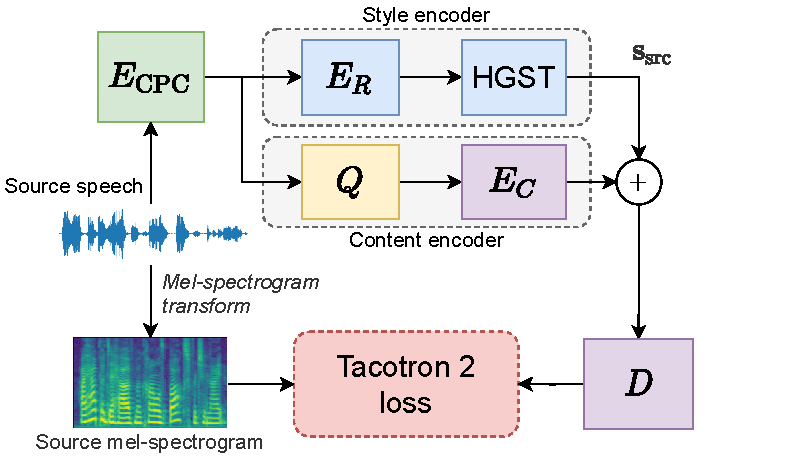
\includegraphics[width=1\textwidth,trim={0.0cm 0cm 0.0cm -0.0cm},clip]{figures/HGST12_training.pdf}
    % %     \end{center}
        
    % %     \column{.52\textwidth}
    % %     \begin{center}
    % %         Inference setup
    % %         \vspace*{0.7cm}
    % %         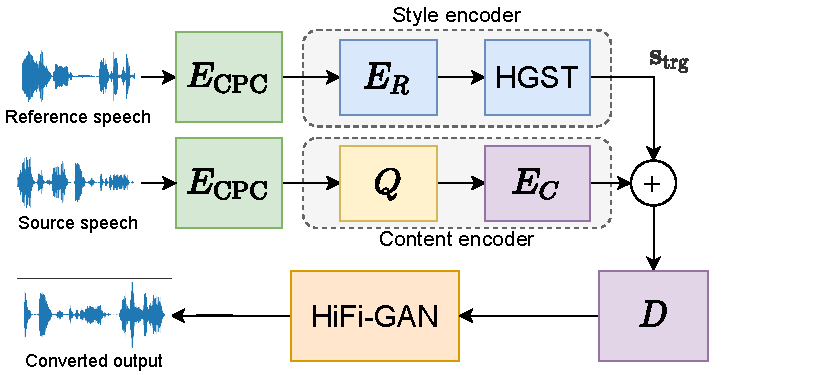
\includegraphics[width=1\textwidth, trim={0cm 0cm 0.0cm -0.0cm},clip]{figures/HGST12_inference.pdf}
    % %     \end{center}
        
    % %     \column{.01\textwidth}
    % % \end{columns}
    % Feed different utterances into style and content encoder branches $\implies$ output obtains speaker from style encoder, linguistic content from content encoder.
\end{block}

% \vfill

% ================================
%  StarGAN-ZSVC
% ================================
% \begin{block}{Cross-lingual augmentation setup}
%     % \vspace*{-1.3cm}
%     % \begin{columns}[c]
%     %     \column{.01\textwidth}
        
%     %     \column{.98\textwidth}
%     %     \begin{center}
%     %         \centerline{\includegraphics[width=1\textwidth,trim={0.3cm 0cm 0.3cm 0cm},clip]{fig2/StarGAN-ZSVC.pdf}}
%     %     \end{center}
        
%     %     \column{.01\textwidth}
%     % \end{columns}
%     % \vspace{-2.1cm}
% \end{block}



% \vfill

% ================================
%  Speaker embedding results
% ================================
\begin{block}{Metrics} % {\large (\%)}}

    % \begin{columns}[T]
    %     \begin{column}{.49\linewidth}
    %     \centering
    %     \sisetup{detect-family}
    %     \begin{table}[t]
    %         \renewcommand{\arraystretch}{1.1}
    %         \centering
    %         \caption{Re-synthesis results in terms of
    %         ASR performance on original and converted data.
    %         % The English-trained VC system is applied to
    %         % English, Sepedi and Afrikaans evaluation data.
    %         Lower W/CER (\%) is more intelligible.
    %         }
    %         \footnotesize
    %         \tablecaptionsep
    %         \label{tab:res-resynth}
    %         \begin{tabularx}{0.95\linewidth}{@{}LS[table-format=2.1]S[table-format=2.1]S[table-format=2.1]S[table-format=2.1]S[table-format=2.1]S[table-format=2.1]@{}}
    %         \toprule
    %          & \multicolumn{2}{c}{{English}} & \multicolumn{2}{c}{{Afrikaans}} &  \multicolumn{2}{c}{{Sepedi}} \\
    %         \cmidrule(l){2-3} \cmidrule(l){4-5} \cmidrule(l){6-7}
            
    %         VC Model & {WER} & {CER} & {WER} & {CER} & {WER} & {CER}\\
    %         \midrule
    %         \textit{Original data} & 5.7 & 1.9 & 6.3 & 4.3 & 2.1 & 0.9 \\
    %         \addlinespace
    %         Full model & 20.6 & 9.6 & 32.5 & 11.0 & 20.4 & 9.5  \\
    %         Without HGST & 21.3 & 9.9 & 34.0 & 11.9 & 21.1 & 9.9 \\
    %         Without $Q$ & \ubold 7.1 & \ubold 2.6 & \ubold 17.0 & \ubold 4.6 & \ubold 3.7 & \ubold 1.6 \\
    %         \bottomrule
    %         \end{tabularx}
    %     \end{table}
            
    %     \end{column}

    

    %     \begin{column}{.49\linewidth}
    %     \centering
    %         \sisetup{detect-family}
    %         \begin{table}[t]
    %             \renewcommand{\arraystretch}{1.1}
    %             \centering
    %             \caption{Speaker similarity error rates (\%) -- Lower values
    %             mean converted is closer to reference than source (better~VC).
    %             % indicate that converted utterances are more often closer to the reference speaker than the source speaker (better~VC).
    %             }
    %             \tablecaptionsep
    %             \footnotesize
    %             \label{tab:res-spk-sim}
    %             \begin{tabularx}{0.95\linewidth}{@{}LS[table-format=2.1]S[table-format=2.1]S[table-format=2.1]@{}}
    %             \toprule
    %             VC Model & {English} & {Afrikaans} & {Sepedi} \\
    %             \midrule
    %             Full model & 8.7 & 22.0 & 58.3 \\
    %             Sans HGST & \ubold 2.3 & \ubold 6.9 & \ubold 34.4 \\
    %             Sans $Q$ & 99.7 & 99.8 & 99.9 \\
    %             \bottomrule
    %             \end{tabularx}
    %             % \aftertableskip
    %         \end{table}            
    %         \small
    %         % MOS for zero-shot setting.
    %     \end{column}
    % \end{columns}
    % \vspace{0.3cm}
    % Without HGST: better VC; without $Q$: more intelligible.\\
    % \mybf{Summary}: decent VC and intelligibility when using both HGST and $Q$.
\end{block}


}\end{minipage}
\end{column}



\begin{column}{.33\linewidth}
\centering
\begin{minipage}[T]{.97\textwidth}\parbox[t][\columnheight]{\textwidth}{


% \vfill

% ================================
%  Objective metric results
% ================================
\begin{block}{Results: Phone Segmentation}
    % Extent to which each model satisfies the four practicality requirement:
    
%     \vspace{0.5ex}


% \begin{table}[tb]
%     \renewcommand{\arraystretch}{1.1}
%     \sisetup{detect-family}
%     \centering
%     \caption{
%     WERs (\%) on LibriSpeech test data for ASR models trained
%     with increasing amounts of VC- and SpecAug-augmented data, with and without 4-gram LM~\mbox{decoding.}
%     }
%     \tablecaptionsep
%     \small
%     \label{tab:res-aug-levels}
%     \begin{tabularx}{0.8\linewidth}{@{}LcS[table-format=2.1]@{\hspace{0.15cm}}S[table-format=2.1]@{\hspace{0.15cm}}S[table-format=2.1]S[table-format=2.1]@{\hspace{0.15cm}}S[table-format=2.1]@{\hspace{0.15cm}}S[table-format=2.1]@{}}

%     \toprule
%     & & \multicolumn{3}{c}{{No LM}} & \multicolumn{3}{c}{{LM decoded}} \\
%     \cmidrule(l){3-5} \cmidrule(l){6-8}
    
%     Augmentation & Amount & {10 min} & {1 h} & {10 h} & {10 min} & {1 h} & {10 h} \\
%     \midrule
%     None & 0\% & 47.7	& \ubold 30.4 &	13.4 & 17.4 &	\ubold 10.6 &	\ubold 7.5  \\
%     VC & 100\% & 43.8 &	32.7 &	13.5 & \ubold 17.2 &	11.4 &	7.6 \\
%     VC & 500\% & 43.5 &	34.4 &	14.4 & 17.9 &	11.9 &	8.1 \\
%     SpecAug & 100\% & 44.3 &	31.8 &	\ubold 13.1 & 18.8 &	11.2 &	7.6 \\
%     SpecAug & 500\% & 43.1 &	34.4 &	13.3 & 17.7	& 12.1 &	7.7 \\
%     VC$\rightarrow$SpecAug & 100\%  & 42.5 & 31.3 &	13.2 & 18.5 &	11.2 &	7.6 \\
%     VC$\rightarrow$SpecAug & 500\%  & \ubold 42.4 &	35.0 &	14.2 & 18.4	& 12.5 &	8.1 \\
%     \bottomrule
%     \end{tabularx}
%     % \aftertableskip
% \end{table}
% \vspace{0.5cm}
% \mybf{Insight:} augmentation only helps when we have very poor \zeroshot{speaker diversity} $\implies$ only helps in very low-resource settings with $\sim$  \nonparallel{10~min of labelled data}.

%     \begin{center}
%         \small
% %         \begingroup
%         \mytable
%         \begin{table}[!hb]
%             \centering
%             \renewcommand{\arraystretch}{1.1}
%             \small
%             \begin{tabular}{l@{\hspace{0.4cm}}p{5.5cm} @{\hspace{0.4cm}}p{4.5cm}@{\hspace{0.4cm}}p{8.5cm}@{\hspace{0.5cm}}l}
        
%             \toprule
%             Model & Non-parallel trainable & Zero-shot capable & Performance in low-resource setting & Speed \\
%             \midrule
%             Linear & \textcolor{softred}{No} & \textcolor{softred}{No} & \textcolor{softred}{Very poor} & \textcolor[HTML]{19a822}{Very fast}\\
%             UNet & \textcolor{softred}{No} & \textcolor{softred}{No} & \textcolor[HTML]{c6341d}{Poor} & \textcolor{softred}{Very slow} \\
%             DBLSTM & \textcolor{softred}{No} & \textcolor{softred}{No} & \textcolor[HTML]{e87000}{Marginally poor} & \textcolor[HTML]{e87000}{Marginally slow}\\
%             StarGAN-VC2 & \textcolor{softgreen}{Yes} & \textcolor{softred}{No} & \textcolor[HTML]{b7b700}{Moderate} & \textcolor[HTML]{b7b700}{Moderate} \\
%             AutoVC & \textcolor{softgreen}{Yes} & \textcolor{softgreen}{Yes} & \textcolor[HTML]{b7b700}{Moderate} & \textcolor[HTML]{e87000}{Marginally slow}\\
%             StarGAN-ZSVC & \textcolor{softgreen}{Yes} & \textcolor{softgreen}{Yes} & \textcolor[HTML]{19a822}{Good} & \textcolor[HTML]{34ba07}{Fast} \\
%             \bottomrule
%             \end{tabular}
%         \end{table}
% %         \endgroup
%     \end{center}

%     \vspace{-1.5ex}
\end{block}

% ================================
%  Mean opinion scores
% ================================
\begin{block}{Results: Cluster quality}

% \begin{table}[!t]
%     \renewcommand{\arraystretch}{1.1}
%     \centering
%     \sisetup{detect-family}
%     \caption{ASR results (\%) on test data of four low-resource languages when trained on  \nonparallel{10 min} of real audio data and different amounts of additional VC- and combined VC-SpecAug augmented data. Sepedi$^*$ uses a non-default training procedure.
%     }
%     \tablecaptionsep
%     \small
%     \label{tab:res-zs}
%     \begin{tabularx}{0.6\linewidth}{@{}l@{\hspace{0.8cm}}Lc@{\hspace{0.8cm}}c@{\hspace{0.8cm}}c@{}}
    
%     \toprule
%     Language & Augmentation & Amount & WER & CER \\
%     \midrule
%     \multirow{3}{*}{Afrikaans}
%     & None                    & 0\% & 52.3 & 15.9 \\
%     & VC                      & 100\% & \ubold 48.9 & \ubold 15.0 \\ 
%     % & VC                      & 500\% & 61.5 & 19.5 \\
%     & VC$\rightarrow$SpecAug  & 100\% & 53.5 & 16.5 \\
%     % & VC$\rightarrow$SpecAug  & 500\% & 83.9 & 33.1 \\
%     % & SpecAug                 & 100\% & 73.9 & 25.3 \\
%     \midrule
%     \multirow{3}{*}{Setswana} 
%     & None                    & 0\% & 68.9 & 26.1 \\
%     & VC                      & 100\% & \ubold 65.9 & \ubold 25.1 \\ 
%     % & VC                      & 500\% & 78.2 & 31.1 \\
%     & VC$\rightarrow$SpecAug  & 100\% & 69.3 & 26.8 \\
%     % & VC$\rightarrow$SpecAug  & 500\% & 87.0 & 40.3 \\
%     \midrule
%     \multirow{3}{*}{isiXhosa}
%     & None                    & 0\% & 63.2 & 15.5 \\
%     & VC                      & 100\% & \ubold  56.5 & \ubold 13.8 \\ 
%     % & VC                      & 500\% & 65.0 & 16.4 \\
%     & VC$\rightarrow$SpecAug  & 100\% & 69.3 & 26.8 \\
%     % & VC$\rightarrow$SpecAug  & 500\% & 89.4 & 28.2 \\
%     \midrule
%     \multirow{3}{*}{Sepedi*}
%     & None                    & 0\% & 92.6 & 50.7 \\
%     & VC                      & 100\% & \ubold 52.8 & \ubold 19.9 \\ 
%     % & VC                      & 500\% & 56.4 & 21.5 \\
%     & VC$\rightarrow$SpecAug  & 100\% & 97.8 & 69.1 \\
%     % & VC$\rightarrow$SpecAug  & 500\% & 98.4 & 73.7 \\
%     \bottomrule
%     \end{tabularx}
%     % \aftertableskip
% \end{table}
% \footnotesize{* different training configuration to allow training convergence.}
\end{block}

% \vfill
% ================================
% Conclusions
% ================================
\begin{block}{Conclusions}
\vspace{-0.23cm}
\begin{itemize}
    \setlength{\itemsep}{0.5ex}
    \item Conclusion content
    % \item VC can be used for data augmentation to improve ASR, but primarily in \nonparallel{very low-resource settings} with limited speaker diversity.
    % \item Cross-lingual VC to drastically different languages unseen during training works well enough to improve ASR performance.
    % \item \mybf{Future}: while our cross-lingual VC augmentation is complementary with SpecAugment, how does it compare/combine with other forms of augmentation? And how well do different VC systems work for cross-lingual VC to unseen languages?
    % % \item No existing model satisfies all practicality requirements.
    % % \item StarGAN-ZSVC better satisfies the requirements, but still not perfect.
    % % \item \mybf{Future:} apply VC systems to practical downstream applications.


\end{itemize}
\end{block}



}\end{minipage}
\end{column}



\begin{column}{.01\linewidth}\end{column} % border column

\end{columns}
\end{frame}

\end{document}